%%
%% This is file `sigconf.tex',
%% generated with the docstrip utility.
%%
%% The original source files were:
%%
%% samples.dtx  (with options: `all,proceedings,sigconf')
%% 
%% IMPORTANT NOTICE:
%% 
%% For the copyright see the source file.
%% 
%% Any modified versions of this file must be renamed
%% with new filenames distinct from sigconf.tex.
%% 
%% For distribution of the original source see the terms
%% for copying and modification in the file samples.dtx.
%% 
%% This generated file may be distributed as long as the
%% original source files, as listed above, are part of the
%% same distribution. (The sources need not necessarily be
%% in the same archive or directory.)
%%
%%
%% Commands for TeXCount
%TC:macro \cite [option:text,text]
%TC:macro \citep [option:text,text]
%TC:macro \citet [option:text,text]
%TC:envir table 0 1
%TC:envir table* 0 1
%TC:envir tabular [ignore] word
%TC:envir displaymath 0 word
%TC:envir math 0 word
%TC:envir comment 0 0
%%
%% The first command in your LaTeX source must be the \documentclass
%% command.
%%
%% For submission and review of your manuscript please change the
%% command to \documentclass[manuscript, screen, review]{acmart}.
%%
%% When submitting camera ready or to TAPS, please change the command
%% to \documentclass[sigconf]{acmart} or whichever template is required
%% for your publication.
%%
%%
\documentclass[sigconf]{acmart}
%%
%% \BibTeX command to typeset BibTeX logo in the docs
\AtBeginDocument{%
  \providecommand\BibTeX{{%
    Bib\TeX}}}

%% Rights management information.  This information is sent to you
%% when you complete the rights form.  These commands have SAMPLE
%% values in them; it is your responsibility as an author to replace
%% the commands and values with those provided to you when you
%% complete the rights form.
\setcopyright{acmlicensed}
\copyrightyear{2027}
\acmYear{2027}
\acmDOI{XXXXXXX.XXXXXXX}
%% These commands are for a PROCEEDINGS abstract or paper.
\acmConference[ACM ASIACCS '27]{}{July 12--16, 2027}{Macau}
%%
%%  Uncomment \acmBooktitle if the title of the proceedings is different
%%  from ``Proceedings of ...''!
%%
%%\acmBooktitle{Woodstock '18: ACM Symposium on Neural Gaze Detection,
%%  June 03--05, 2018, Woodstock, NY}
% \acmISBN{978-1-4503-XXXX-X/2018/06}


%%
%% Submission ID.
%% Use this when submitting an article to a sponsored event. You'll
%% receive a unique submission ID from the organizers
%% of the event, and this ID should be used as the parameter to this command.
\acmSubmissionID{123-A56-BU3} %%%%%%%%%%%%%%%%%%%%%%%%%%%%%%%%%%%%%%%%%%%%%%%%%%%%%%%%%%%

%%
%% For managing citations, it is recommended to use bibliography
%% files in BibTeX format.
%%
%% You can then either use BibTeX with the ACM-Reference-Format style,
%% or BibLaTeX with the acmnumeric or acmauthoryear sytles, that include
%% support for advanced citation of software artefact from the
%% biblatex-software package, also separately available on CTAN.
%%
%% Look at the sample-*-biblatex.tex files for templates showcasing
%% the biblatex styles.
%%
%%
%% The majority of ACM publications use numbered citations and
%% references.  The command \citestyle{authoryear} switches to the
%% "author year" style.
%%
%% If you are preparing content for an event
%% sponsored by ACM SIGGRAPH, you must use the "author year" style of
%% citations and references.
%% Uncommenting
%% the next command will enable that style.
%%\citestyle{acmauthoryear}
\usepackage{array}

%%
%% end of the preamble, start of the body of the document source.
\begin{document}

%%
%% The "title" command has an optional parameter,
%% allowing the author to define a "short title" to be used in page headers.
\title{TAILGUARD: An Uncertainty-Driven Ensemble
Against Long-Tailed Cyber Threats}

%%
%% The "author" command and its associated commands are used to define
%% the authors and their affiliations.
%% Of note is the shared affiliation of the first two authors, and the
%% "authornote" and "authornotemark" commands
%% used to denote shared contribution to the research.
\author{Anonymous}
% \authornote{Both authors contributed equally to this research.}
% \email{trovato@corporation.com}
% \orcid{1234-5678-9012}
% \author{G.K.M. Tobin}
% \correspondingauthor
% \authornotemark[1]
% \email{webmaster@marysville-ohio.com}
% \affiliation{%
%   \institution{Institute for Clarity in Documentation}
%   \city{Dublin}
%   \state{Ohio}
%   \country{USA}
% }

% \author{Lars Th{\o}rv{\"a}ld}
% \affiliation{%
%   \institution{The Th{\o}rv{\"a}ld Group}
%   \city{Hekla}
%   \country{Iceland}}
% \email{larst@affiliation.org}

% \author{Valerie B\'eranger}
% \affiliation{%
%   \institution{Inria Paris-Rocquencourt}
%   \city{Rocquencourt}
%   \country{France}
% }

% \author{Aparna Patel}
% \affiliation{%
%  \institution{Rajiv Gandhi University}
%  \city{Doimukh}
%  \state{Arunachal Pradesh}
%  \country{India}}

% \author{Huifen Chan}
% \affiliation{%
%   \institution{Tsinghua University}
%   \city{Haidian Qu}
%   \state{Beijing Shi}
%   \country{China}}

% \author{Charles Palmer}
% \affiliation{%
%   \institution{Palmer Research Laboratories}
%   \city{San Antonio}
%   \state{Texas}
%   \country{USA}}
% \email{cpalmer@prl.com}

% \author{John Smith}
% \affiliation{%
%   \institution{The Th{\o}rv{\"a}ld Group}
%   \city{Hekla}
%   \country{Iceland}}
% \email{jsmith@affiliation.org}

% \author{Julius P. Kumquat}
% \correspondingauthor
% \affiliation{%
%   \institution{The Kumquat Consortium}
%   \city{New York}
%   \country{USA}}
% \email{jpkumquat@consortium.net}

%%
%% By default, the full list of authors will be used in the page
%% headers. Often, this list is too long, and will overlap
%% other information printed in the page headers. This command allows
%% the author to define a more concise list
%% of authors' names for this purpose.
% \renewcommand{\shortauthors}{Trovato et al.}

%%
%% The abstract is a short summary of the work to be presented in the
%% article.
\begin{abstract}
TBD
\end{abstract}

%%
%% The code below is generated by the tool at http://dl.acm.org/ccs.cfm.
%% Please copy and paste the code instead of the example below.
%%

\begin{CCSXML}
<ccs2012>
 <concept>
  <concept_id>00000000.0000000.0000000</concept_id>
  <concept_desc>Do Not Use This Code, Generate the Correct Terms for Your Paper</concept_desc>
  <concept_significance>500</concept_significance>
 </concept>
 <concept>
  <concept_id>00000000.00000000.00000000</concept_id>
  <concept_desc>Do Not Use This Code, Generate the Correct Terms for Your Paper</concept_desc>
  <concept_significance>300</concept_significance>
 </concept>
 <concept>
  <concept_id>00000000.00000000.00000000</concept_id>
  <concept_desc>Do Not Use This Code, Generate the Correct Terms for Your Paper</concept_desc>
  <concept_significance>100</concept_significance>
 </concept>
 <concept>
  <concept_id>00000000.00000000.00000000</concept_id>
  <concept_desc>Do Not Use This Code, Generate the Correct Terms for Your Paper</concept_desc>
  <concept_significance>100</concept_significance>
 </concept>
</ccs2012>
\end{CCSXML}

\ccsdesc[500]{Do Not Use This Code~Generate the Correct Terms for Your Paper}
\ccsdesc[300]{Do Not Use This Code~Generate the Correct Terms for Your Paper}
\ccsdesc{Do Not Use This Code~Generate the Correct Terms for Your Paper}
\ccsdesc[100]{Do Not Use This Code~Generate the Correct Terms for Your Paper}

%% A "teaser" image appears between the author and affiliation
%% information and the body of the document, and typically spans the
%% page.
% \begin{teaserfigure}
%  \includegraphics[width=\textwidth]{sampleteaser}
%   \caption{Seattle Mariners at Spring Training, 2010.}
%   \Description{Enjoying the baseball game from the third-base
%   seats. Ichiro Suzuki preparing to bat.}
%   \label{fig:teaser}
% \end{teaserfigure}

\received{21 August 2026}
% \received[revised]{12 March 2009}
% \received[accepted]{5 June 2009}

%%
%% This command processes the author and affiliation and title
%% information and builds the first part of the formatted document.
\maketitle

\section{Introduction}
Network Intrusion Detection Systems (NIDS) deployed in practice must satisfy two requirements at once: classify a network flow into the correct known attack family with enough granularity to inform a response, and recognize when a flow belongs to an attack type absent from training altogether, rather than silently forcing it into the nearest known class \citep{liu2019machine}. The first requirement is closed-set, $|C|$-way classification; the second is open-set by nature, since no closed-set classifier -- however accurate on the classes it was shown -- has any mechanism for the case it was not. Both are made harder by a property shared across NIDS benchmarks: real network traffic is severely long-tailed \citep{wang2020long}. Across the four NetFlow-v3 (NF-v3) benchmarks \citep{luay2025NetFlowDatasetsV3} used in this work (Section~\ref{data}), per-dataset Imbalance Ratio \citep{Zhong_2021_CVPR} ranges from 4,228 to 14,163; in CSE-CIC-IDS2018 alone, Benign traffic accounts for 17,514,626 flows (87.07\%) while Web Attacks -- one of the classes an operator most needs to catch -- has only 2,538 (0.0126\%). This imbalance does not merely bias closed-set accuracy toward the head class: it starves precisely the tail classes of the samples needed to characterize both their decision boundary and their in-distribution support, which is exactly what the open-set requirement depends on. A NIDS that handles long-tailed known classes well but cannot reject unseen ones, or vice versa, has not solved the deployment problem -- it has only relocated where it fails.

Existing IDS work addresses these two requirements only partially. Classical tabular approaches -- gradient-boosted tree ensembles such as XGBoost \citep{chen2016xgboost}, which remain highly competitive on flow-level tabular features \citep{grinsztajn2022tree,zhou2020building} -- are typically trained and evaluated closed-set, with no mechanism for rejecting a class outside their label set. A more recent line of representation-learning IDS work, spanning graph neural networks \citep{lo_e-graphsage_2022,caville_anomal-e_2022,xu_negsc_2024,nguyen_ts-ids_2023} and transformer architectures \citep{manocchio_flowtransformer_2024,han_gtid_2023}, improved on parts of this picture, but -- as Section~\ref{sec:existing} details -- largely by narrowing the task: several of the strongest reported results are for binary benign-versus-attack detection \citep{caville_anomal-e_2022,zhang_aoc-ids_2024} or coarse, few-class taxonomies \citep{han_gtid_2023} rather than the full per-attack-type, long-tailed multi-class problem. Multi-class, per-attack-type classification that is also open-set -- naming a known attack family correctly while explicitly rejecting an unseen one -- remains comparatively underexplored across both lines of work.

We close this gap with an independent-expert architecture that resolves both requirements through the same mechanism, rather than bolting an open-set check onto a closed-set classifier after the fact. Instead of a single shared, learned gate that must route a sample correctly before its designated expert can act on it, we partition known attack classes by taxonomy into disjoint groups and train one expert per group -- plus a further expert dedicated to benign traffic, on equal footing with every attack family -- entirely independently, each equipped with its own Energy-based accept/reject gate \citep{liu2020energy} (Section~\ref{sec:approach}). Because every expert only has to discriminate within its own, substantially smaller class pool rather than the full $|C|$-way label space, even a sparsely populated tail attack family faces an easier local decision boundary than it would inside one global classifier. The same Energy gate that resolves this narrower classification problem also supplies the open-set signal: a flow that no expert -- including the benign expert -- accepts is predicted unseen (Section~\ref{ssec:routing}), which is what lets the architecture generalize under open-world conditions and genuine distribution shift, not only within the class set it was trained on. We pair this with cross-dataset auxiliary OOD exposure, made free by the fact that all four NF-v3 datasets share an identical 46-feature schema (Section~\ref{ssec:expert-design}), and with an evaluation protocol that holds out entire attack classes from training, validation, and threshold calibration rather than resampling a class the model has already seen (Section~\ref{sec:openset}).

\paragraph{Contributions}
\begin{itemize}
    \item \textbf{An independent-expert, Energy-gated architecture for open-set IDS.} We partition known attack classes by attack-family taxonomy into experts trained entirely independently, each with its own Energy-based accept/reject gate (Section~\ref{ssec:ood-gating}) in place of a shared, learned router -- so that each expert discriminates within its own, substantially smaller class pool rather than the full $|C|$-way label space, giving even sparsely populated tail classes an easier local decision boundary. Benign traffic is trained as one more such expert rather than handled as a fixed reference point (Section~\ref{ssec:expert-design}): to our knowledge, no prior IDS design treats ``is this benign'' as just another expert-level accept/reject decision, on equal footing with ``is this attack family $k$.''
    \item \textbf{Cross-dataset auxiliary OOD exposure and an open-world, genuinely unseen-class evaluation protocol.} The NF-v3 schema's identical 46-feature representation across four IDS benchmarks (Section~\ref{data}) lets each expert's OOD gate train on attack traffic from the \emph{other} three datasets at no feature-alignment cost (Section~\ref{ssec:expert-design}). We pair this with an open-set evaluation that holds out entire attack classes from training, validation, and threshold calibration (Section~\ref{sec:openset}), rather than a resampled split of a class the model has already seen, so that reported OOD performance reflects genuine distribution shift rather than an easier, already-seen-class holdout.
    \item \textbf{An explicit accounting of what a confidence-only routing rule can and cannot resolve.} The Multi-IN resolution rule (Section~\ref{ssec:routing}) reduces at $\lambda=0$ to selecting the lowest-Energy accepting expert with no learned router or test-time perturbation. We characterize where this simple rule suffices and where it structurally cannot -- e.g. when two classes are genuinely close in feature space rather than merely miscalibrated at the decision threshold (Section~\ref{ssec:ablation}) -- giving an empirical basis for whether the stability extension ($\lambda>0$) is worth pursuing, instead of assuming it a priori.
\end{itemize}

\section{Background}
\subsection{Intrusion Detection Systems}
\label{IDS}
Intrusion Detection Systems (IDS) monitor events observed in hosts or networks to detect signs of intrusion. According to \cite{liu2019machine}, IDS can be categorized from an analytical perspective into misuse detection and anomaly detection. Misuse detection is advantageous for precise identification of known attack patterns but vulnerable to zero-day attacks, while anomaly detection leverages statistical deviations from normal behavior profiles to detect unknown attacks. Based on data sources, IDS can be divided into Host-based IDS (HIDS) and Network-based IDS (NIDS), where HIDS primarily observes internal host behaviors such as system logs and system calls, while NIDS monitors network traffic. A network flow is a sequence of packets sharing common characteristics such as source and destination IP addresses, port numbers, and protocol type \citep{moustafa2015unsw}; NIDS typically operate on such flow-level features aggregated from raw packet captures, rather than on individual packets or payloads. In this work, we study anomaly-detection-based NIDS operating on the flow-based feature representations detailed for each dataset in Section~\ref{data}, including UNSW-NB15~\citep{moustafa2015unsw} and CSE-CIC-IDS2018~\citep{sharafaldin2018toward}.

\subsection{Long-tailed Distribution}
Long-tailed distributions, in which a small number of head classes dominate the sample count while the majority of classes are severely under-represented, are pervasive in real-world data \citep{wang2020long}. Such imbalance biases model training toward head classes and undermines both closed-set classification and out-of-distribution (OOD) detection, since tail classes provide too few samples to reliably characterize either their decision boundary or their in-distribution support. This effect is particularly severe for IDS: as detailed in Section~\ref{data}, in CSE-CIC-IDS2018 the majority class (Benign) accounts for 17,514,626 samples (87.07\% of the dataset), whereas the smallest attack class (Web Attacks) contains only 2,538 samples (approximately 0.0126\%) -- and it is precisely these rare, under-represented classes that an IDS most needs to detect.

\textbf{Imbalance Ratio (IR)} \citep{Zhong_2021_CVPR} is defined as:
\begin{equation}
\text{IR} = \frac{n_{\max}}{n_{\min}}
\end{equation}
where $n_{\max}$ and $n_{\min}$ are the maximum and minimum class sample counts, respectively.

In addition to quantifying imbalance, IR is used as a controllable variable in controlled studies. Researchers often start with an originally balanced dataset and artificially apply a target IR (e.g., CIFAR-10/100-LT) composed of specific imbalance coefficients, thereby fixing the domain and task and isolating the impact of imbalance severity. 
%%# Add existing LT methods briefly?



\subsection{Mixture-of-Experts (MoE) Architecture}
MoE architecture is a widely adopted ensemble learning paradigm where multiple specialized models, termed ``experts,'' are trained to classify different subsets of the input space. Given an input $x$, a set of $K$ expert networks $\{f_k\}_{k=1}^{K}$, and a gating network $g$, the MoE output is a weighted combination of the expert outputs:
\begin{equation}
y = \sum_{k=1}^{K} g_k(x) \cdot f_k(x)
\end{equation}
where $g_k(x)$ is the $k$-th component of the gating weight vector $g(x) \in \Delta^{K-1}$, satisfying $\sum_{k=1}^{K} g_k(x) = 1$ and $g_k(x) \geq 0$. Unlike conventional ensembles, which combine all constituent models with fixed, input-independent weights, MoE employs \textit{conditional computation}: $g(x)$ is itself a learned function of the input, allowing different experts to specialize in different regions of the input space \citep{jordan1994hierarchical}. Depending on how $g(x)$ is computed and how many experts are activated per input, MoE architectures fall into three broad categories.

\textbf{Soft (Dense) MoE.} In the original formulation \citep{jacobs1991adaptive, jordan1994hierarchical}, the gating network activates all $K$ experts for every input, with $g(x)$ computed as a softmax over a learned linear projection of $x$:
\begin{equation}
g(x) = \mathrm{Softmax}(xW_g), \qquad g_k(x) = \frac{\exp\big((xW_g)_k\big)}{\sum_{j=1}^{K}\exp\big((xW_g)_j\big)}
\end{equation}
where $W_g \in \mathbb{R}^{d \times K}$ is the gating weight matrix. Because every expert contributes to every prediction, dense MoE incurs the full inference cost of all $K$ experts and provides no explicit mechanism for rejecting an expert's contribution.

\textbf{Sparse (Top-$k$) MoE.} To reduce computation and encourage specialization, \citet{shazeer2017outrageously} restrict $g(x)$ to its top-$k$ components ($k \ll K$), zeroing out the rest before renormalization, and inject tunable noise for load balancing across experts:
\begin{equation}
g(x) = \mathrm{Softmax}\big(\mathrm{KeepTopK}(H(x), k)\big)
\end{equation}
\begin{equation}
    \qquad H(x) = xW_g + \epsilon \cdot \mathrm{Softplus}(xW_{\mathrm{noise}})
\end{equation}
where $\epsilon \sim \mathcal{N}(0, I)$ and $\mathrm{KeepTopK}(v, k)$ sets all but the $k$ largest entries of $v$ to $-\infty$ (so that $\mathrm{Softmax}$ assigns them zero weight). Only the selected experts are evaluated at inference time, making sparse MoE the standard choice for scaling to large expert counts.

\textbf{Hard-routing MoE.} In the limiting case $k=1$, the gate collapses to a deterministic, argmax selection of a single expert:
\begin{equation}
r(x) = \arg\max_{k \in \{1,\dots,K\}} g_k(x), \qquad y = f_{r(x)}(x)
\end{equation}
i.e., the gating weight vector degenerates to a one-hot indicator, $g_k(x) = \mathbb{1}[k = r(x)]$, and the final prediction is produced exclusively by the selected expert. This specialization is crucial in long-tailed classification tasks, as it allows individual experts to focus on specific, often sparse, tail-class distributions, thereby mitigating the bias toward head classes \citep{wang2020long}. In the context of intrusion detection, where benign traffic dominates the dataset and attack classes exhibit substantial distributional diversity, the MoE framework enables each expert to focus on specific attack types or behavioral patterns.

Our model adopts this hard-routing formulation with a class-aware router: rather than learning $r(x)$ purely to minimize a load-balancing or reconstruction objective, the router selects the expert that owns the class of $x$, so that $r(x)$ is defined by the class-to-expert ownership partition described in Section~\ref{sec:approach}.%%# Can be revised according to the model architecture

\section{Existing Intrusion Detection}
\label{sec:existing}
\paragraph{GNN-based}
A substantial line of recent IDS work represented network flows as graphs, with hosts as nodes and flows as edges, and applied graph neural networks (GNNs) to the resulting structure.

\textbf{E-GraphSAGE} \citep{lo_e-graphsage_2022} constructed a graph in which each node corresponded to an IP address and each directed edge corresponded to a flow between two hosts, with the edge feature vector built from flow-level statistics such as TCP flags, byte counts, protocol, and duration. An edge-embedding variant of GraphSAGE then aggregated neighboring edge features to classify each flow. E-GraphSAGE was evaluated on the NF-* NetFlow-unified datasets and became the de facto baseline against which the GNN-based IDS line that followed it compared itself.

\textbf{Anomal-E} \citep{caville_anomal-e_2022} replaced E-GraphSAGE's supervised training with a self-supervised objective, using Deep Graph Infomax to learn edge embeddings without attack labels and scoring anomalies from the learned representation. This removed the dependence on labeled attack data, but in doing so reduced the task to a binary, benign-versus-attack decision; Anomal-E did not report per-attack-type classification.

\textbf{NEGSC} \citep{xu_negsc_2024} combined a self-supervised GNN encoder with a graph contrastive loss and reported both binary and multi-class results on NF-BoT-IoT and NF-CSE-CIC-IDS2018, directly comparing against Anomal-E, several tree-based classifiers, and TS-IDS.

\textbf{TS-IDS} \citep{nguyen_ts-ids_2023} extended this line with a traffic-aware self-supervised GNN evaluated across all four NF-v2 NetFlow-unified datasets used in this work (NF-UNSW-NB15-v2, NF-CSE-CIC-IDS2018-v2, NF-BoT-IoT, NF-ToN-IoT) and reported multi-class, per-class performance against XGBoost, E-GraphSAGE, and Anomal-E, making it the closest existing multi-class GNN baseline to our setting.

\paragraph{Transformer-based}
A separate line of work applied transformer architectures to flow- or packet-sequence representations of network traffic.

\textbf{FlowTransformer} \citep{manocchio_flowtransformer_2024} proposed a modular transformer framework for flow-based NIDS that allowed the input encoding, transformer block, and classification head to be swapped independently. Its released implementation, however, used a single sigmoid output trained with binary cross-entropy -- a binary detector rather than a multi-class classifier, despite the framework's claimed flexibility.

\textbf{GTID} \citep{han_gtid_2023} combined n-gram frequency features with a time-aware transformer and evaluated a three-class classification setting (benign plus two coarse attack groups), a substantially coarser taxonomy than the per-attack-type classification considered in this work.

\paragraph{Contrastive-based}
Beyond graph- and transformer-specific architectures, several IDS adopted contrastive or self-supervised objectives to cope with limited or imbalanced attack labels. 

\textbf{AOC-IDS} \citep{zhang_aoc-ids_2024} paired an autoencoder with a cluster-repelling contrastive loss in an online learning setting, continuously updating its behavior profile as new traffic arrived; as with Anomal-E, its evaluation targeted anomaly (benign-versus-attack) detection rather than attack-type classification.

\paragraph{Tabular Foundation Models}
TBD

Taken together, this body of work showed that GNN- and transformer-based IDS made substantial progress on binary or coarse-grained detection, while multi-class, per-attack-type classification under severe long-tailed imbalance -- the setting we study in Section~\ref{sec:approach} -- remained comparatively underexplored. TS-IDS and NEGSC are the closest existing points of comparison and are the SOTA baselines we adopt in Section~\ref{data}.

\section{Proposed Approach}
\label{sec:approach}
We propose an independent-expert architecture for open-set, OOD-aware classification of long-tailed IDS traffic. Rather than training a single monolithic classifier over all classes, we partition the known attack taxonomy of a target dataset into disjoint groups and train one expert per group, plus one additional expert dedicated to benign traffic, entirely independently of one another (Section~\ref{ssec:expert-design}). Each expert learns to accept or reject an input via an Energy-based OOD score before ever attempting to classify it (Section~\ref{ssec:ood-gating}); at test time, every expert evaluates every input in parallel, and the number of experts that accept it -- not any single expert's confidence in isolation -- determines how the final prediction is resolved (Section~\ref{ssec:routing}). Figure~\ref{fig:architecture} summarizes both stages.

\begin{figure*}[t]
\centering
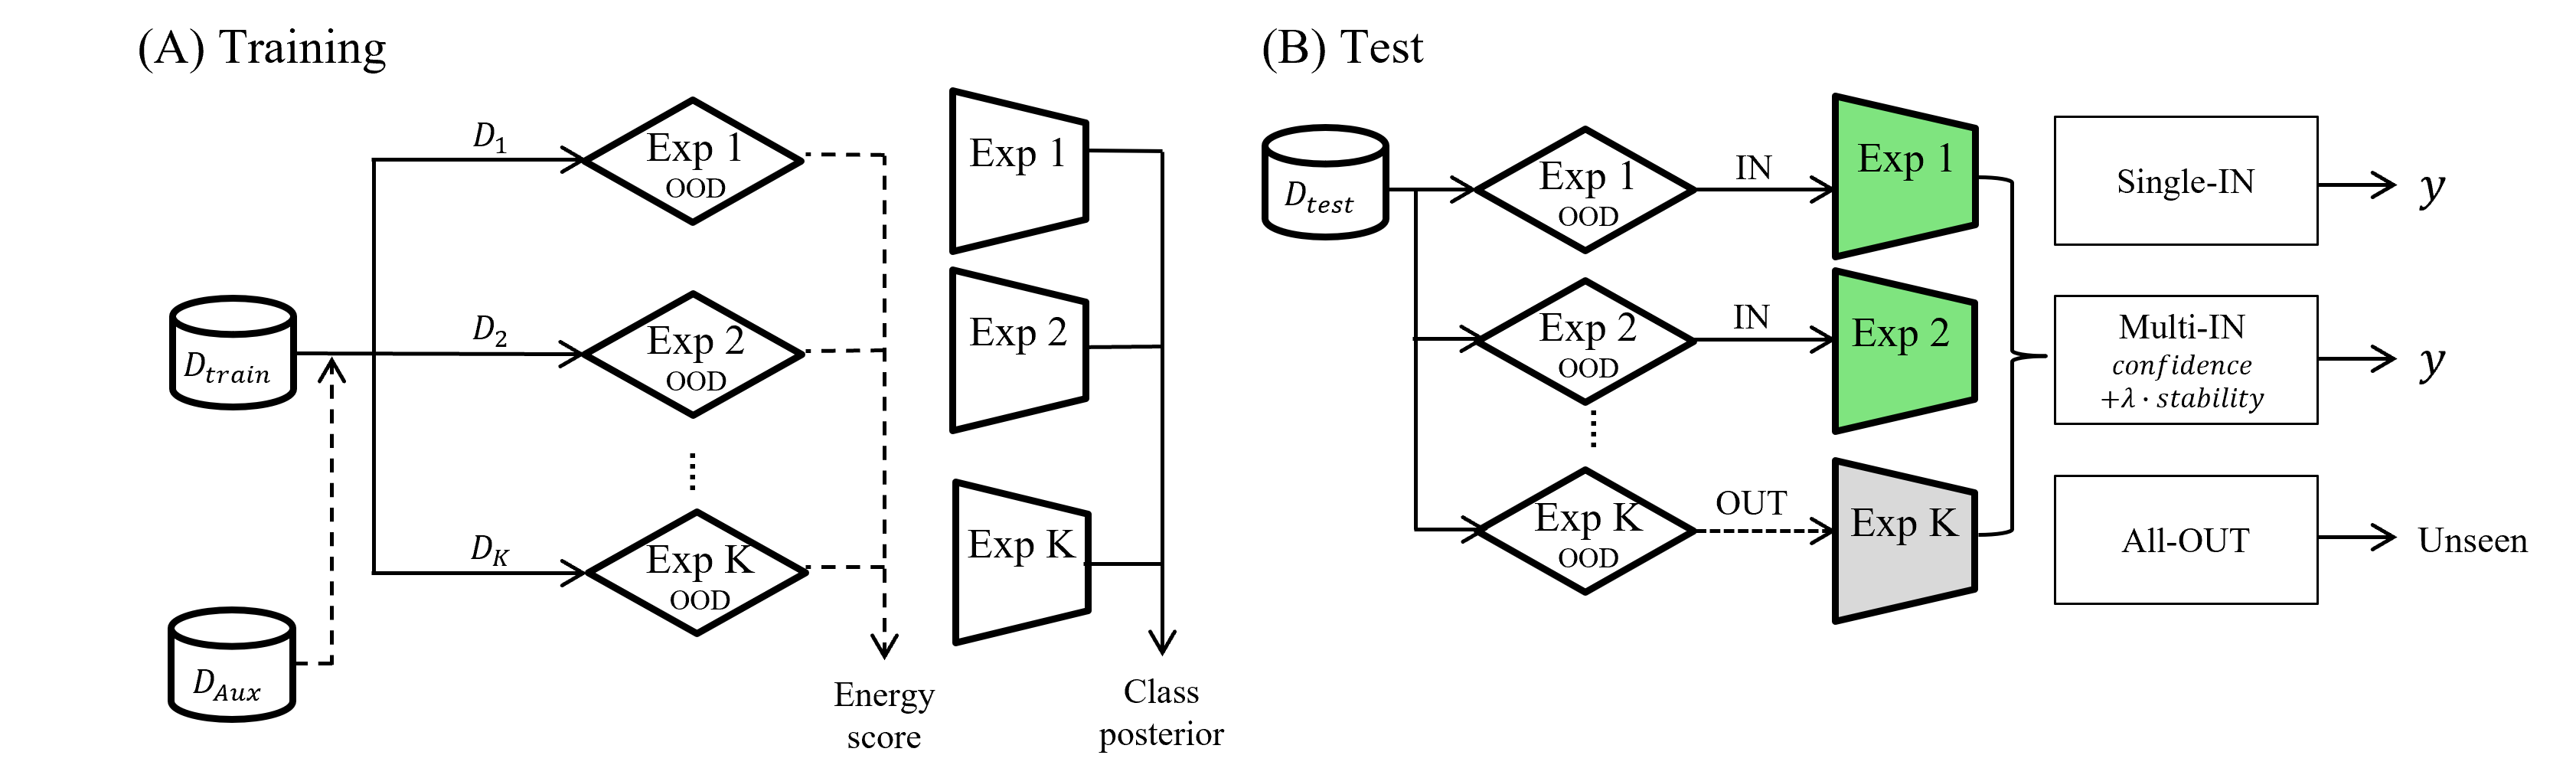
\includegraphics[width=\textwidth]{figures/mainfig.png}
\caption{Independent expert design. (A) Training: the known attack classes of a target dataset are partitioned into $D_0, \ldots, D_K$ by attack-family taxonomy (Section~\ref{ssec:expert-design}; e.g., for CSE-CIC-IDS2018, $D_0 = \text{Flood} = \{\text{DDoS}, \text{DoS}\}$). Each attack expert $k$ trains an XGBoost classifier on its owned classes $D_k$ only, and separately trains an energy-margin MLP on $D_k$ (ID) versus every other known class plus external cross-dataset auxiliary data $D_{\mathrm{Aux}}$ (OOD) to obtain an accept/reject energy score (Section~\ref{ssec:ood-gating}). A benign expert is trained identically, with $D_{\mathrm{benign}}$ as its ID set and $\bigcup_{k} D_k$ (every known attack class) as its OOD set; panel (B) depicts it generically as one of Exp~1,~\ldots,~Exp~K rather than drawing it separately, since it is evaluated by the same accept/reject pipeline as every attack expert. (B) Test-time inference: a single pipeline evaluates every expert in parallel; the number of accepting experts, not the input type, determines the branch (Section~\ref{ssec:routing}). Single-IN is resolved by the accepting expert's classifier. Multi-IN is resolved by $\arg\max_k [\,\mathrm{conf}_k + \lambda \cdot \mathrm{stab}_k\,]$ among the accepting experts; this work uses $\lambda = 0$ (confidence only), with $\lambda > 0$ left as future work (Section~\ref{ssec:routing}). All-OUT means no expert -- including the benign expert -- accepts $x$, so $x$ is predicted unseen.}
\label{fig:architecture}
\end{figure*}

\subsection{Problem Formulation}
Let $\mathcal{D}$ denote a target NIDS dataset (Section~\ref{data}) with a benign class and known attack classes $C = \{c_1, \ldots, c_M\}$. At deployment, a test flow $x$ may belong to a known class in $C \cup \{\text{benign}\}$, or to an attack type absent from $C$ entirely -- an \textit{unseen} class held out from training, validation, and threshold calibration to simulate a genuinely novel attack (Section~\ref{sec:openset}). The task is therefore $(|C|+2)$-way: classify $x$ into one of the $|C|$ known attack classes, into benign, or reject it as unseen. This is strictly harder than the closed-set, $|C|$-way classification that the XGBoost baseline (Section~\ref{data}) solves, since a closed-set classifier has no mechanism for the unseen case by construction and is evaluated only on its known-class accuracy.

\subsection{Independent Expert Design} \label{ssec:expert-design}
Known attack classes are partitioned into $K{+}1$ disjoint groups $D_0, \ldots, D_K$ by attack-family taxonomy, fixed per target dataset (e.g., for CSE-CIC-IDS2018, $D_0 = \text{Flood} = \{\text{DDoS}, \text{DoS}\}$, $D_1 = \text{Brute-Force}$, $D_2 = \text{Tail} = \{\text{Bot}, \text{Infiltration}, \text{Web Attacks}\}$); full per-dataset partitions are given in Appendix~\ref{app:datasets}. Expert $k \in \{0, \ldots, K\}$ is trained with $D_k$ as its in-distribution (ID) set and every other known class as its out-of-distribution (OOD) set,
\begin{equation}
\text{OOD}_k = \Big(\bigcup_{j \neq k} D_j\Big) \cup D_{\mathrm{Aux}},
\end{equation}
where $D_{\mathrm{Aux}}$ is attack traffic drawn from the other three NF-v3 datasets (Section~\ref{data}) whose attack-family semantics do not overlap with $D_k$'s -- an auxiliary outlier-exposure source that costs nothing to collect, since every dataset shares the same 46-feature schema (Section~\ref{data}). Benign traffic is never included in $D_{\mathrm{Aux}}$ or in any $\text{OOD}_k$: mixing it in would make it impossible for the routing stage (Section~\ref{ssec:routing}) to later distinguish ``this expert rejected $x$ because it looks like a different known attack'' from ``this expert rejected $x$ because it looks benign.''

Benign itself is trained as an additional, dedicated expert on exactly the same footing: its ID set is $D_{\mathrm{benign}}$, and its OOD set is every known attack class, $\text{OOD}_{\mathrm{benign}} = \bigcup_{k=0}^{K} D_k$, plus $D_{\mathrm{Aux}}$. This differs from treating benign as a fixed reference point, e.g. thresholding distance to a benign centroid: benign traffic empirically has no compact, centroid-like distribution in this feature space (Section~\ref{sec:discussion}), so a distance-based rule cannot reliably separate it from either known attacks or unseen traffic. Training benign as one more Energy-gated expert instead lets it compete for a sample on equal footing with every attack expert at test time (Section~\ref{ssec:routing}), through the same learned, nonlinear accept/reject mechanism rather than a hand-fit geometric threshold.

Every expert $k \in \{0, \ldots, K\} \cup \{\mathrm{benign}\}$ additionally trains a local classifier $h_k$ on its own ID set (an XGBoost model, following Section~\ref{data}'s baseline, for the $K{+}1$ attack experts; $D_{\mathrm{benign}}$ has only one class, so $h_{\mathrm{benign}}$ is the constant prediction benign), used only when that expert accepts the input (Section~\ref{ssec:routing}).

\subsection{Energy-based OOD Gating} \label{ssec:ood-gating}
Each expert $k$ separately trains an MLP $f_k$ that produces $|D_k|$ class logits (or, for a singleton $D_k$, two logits, with the second an unused placeholder to avoid degenerate one-class cross-entropy), plus an Energy-based accept/reject score computed from those same logits. Given logits $f_k(x)$ and temperature $T$, the Energy of $x$ under expert $k$ is
\begin{equation}
E_k(x) = -T \cdot \log \sum_{i} \exp\big(f_k(x)_i / T\big),
\end{equation}
following \citep{liu2020energy}; lower $E_k(x)$ indicates $x$ is more in-distribution for expert $k$. After an initial supervised pretraining phase on $D_k$ alone, each expert is fine-tuned with a margin loss that explicitly separates ID and OOD energy,
\begin{align}
\mathcal{L}_k = \mathcal{L}_{\mathrm{CE}} &+ \beta \, \mathbb{E}_{x \in D_k} \max(0,\, E_k(x) - m_{\mathrm{in}})^2 \notag \\
&+ \beta \, \mathbb{E}_{x \in \text{OOD}_k} \max(0,\, m_{\mathrm{out}} - E_k(x))^2,
\end{align}
pushing ID energy below $m_{\mathrm{in}}$ and OOD energy above $m_{\mathrm{out}} > m_{\mathrm{in}}$. Margins are set automatically per expert from its pretrained energy distribution on a held-out ID validation split (the mean offset by a fixed multiple of its standard deviation) rather than tuned globally, since ID energy scale varies substantially across experts -- in particular between multi-class and singleton $D_k$. The accept/reject threshold $\tau_k$ used at test time (Section~\ref{ssec:routing}) is calibrated as a fixed quantile of expert $k$'s own ID validation energy, independent of every other expert: $x$ is accepted by expert $k$ iff $E_k(x) \leq \tau_k$.

\subsection{Routing and Final Prediction} \label{ssec:routing}
At test time, every expert independently evaluates $x$ against its own threshold $\tau_k$, producing a set of accepting experts $\mathcal{A}(x) = \{k : E_k(x) \leq \tau_k\}$, $k$ ranging over the $K{+}1$ attack experts and the benign expert. The final prediction is resolved from $|\mathcal{A}(x)|$ alone, with no additional router trained on top:

\textbf{Single-IN} ($|\mathcal{A}(x)| = 1$). The unique accepting expert's local classifier decides: $y = h_k(x)$ for $\mathcal{A}(x) = \{k\}$.

\textbf{Multi-IN} ($|\mathcal{A}(x)| > 1$). We select among the accepting experts by
\begin{equation}
k^\star = \arg\max_{k \in \mathcal{A}(x)} \big[\, \mathrm{conf}_k(x) + \lambda \cdot \mathrm{stab}_k(x) \,\big], \qquad y = h_{k^\star}(x),
\end{equation}
where $\mathrm{conf}_k(x) = -E_k(x)$ and $\mathrm{stab}_k(x)$ is a test-time-perturbation stability score (agreement of $f_k$'s prediction across small perturbations of $x$). At $\lambda = 0$ this reduces to selecting the accepting expert with the lowest Energy, i.e. the one most confident about its own ID region -- the configuration used throughout this work. Adding a stability term ($\lambda > 0$) is motivated by a limitation of the $\lambda = 0$ rule: it resolves Multi-IN correctly when the accepting experts merely straddle each other's decision threshold, but not when the competing classes are genuinely close in feature space, since a non-owning expert can be more confident, not less, about a sample outside its true class. This is close in spirit to test-time-augmentation stability routing explored earlier in this project, which failed because a non-owning expert was found to be just as stable as the true owner when routing was attempted \emph{from scratch} across all experts; here, stability would instead act as a secondary tie-break applied only among experts that have \emph{already} independently passed their own Energy accept test -- a materially smaller and less symmetric candidate set. Whether this narrower use of stability succeeds where the unrestricted version did not is an open question this work has not yet tested; we report $\lambda = 0$ as the primary configuration and leave $\lambda > 0$ to future work.

\textbf{All-OUT} ($|\mathcal{A}(x)| = 0$). No expert -- including the dedicated benign expert -- accepts $x$ as in-distribution for its own class, so $x$ is predicted unseen.


\section{Experiments}
\subsection{Experimental Setup}
\subsubsection{Datasets} \label{data}
As introduced in Section~\ref{IDS}, intrusion detection systems fundamentally operate on network traffic flows, extracting flow-based features from packet captures for subsequent classification. This work uses four benchmark NIDS datasets -- UNSW-NB15, CSE-CIC-IDS2018, BoT-IoT, and ToN-IoT -- re-released under the University of Queensland's unified NetFlow-v3 (NF-v3) schema. All four datasets were originally released with different, tool-specific feature sets; \citep{luay2025NetFlowDatasetsV3} and the same group's earlier NetFlow-unification releases re-extracted them from raw packet captures into a common schema, culminating in NF-v3's 46 usable features, listed in Table~\ref{tab:nfv3_features}: byte/packet/TCP-flag counts and inter-arrival-time statistics per direction, TTL and packet-length extremes, a packet-length histogram, retransmission counts, average throughput, and a few application-layer fields (ICMP, DNS, FTP). This identical feature space across all four datasets, rather than the dataset-specific schemas each was originally released with, is what makes the cross-dataset auxiliary OOD exposure and open-set generalization evaluation in Section~\ref{sec:approach} possible without a feature-alignment step. Testbed configurations and full attack-taxonomy descriptions are given in Appendix~\ref{app:datasets} to keep this section brief.


\begin{table}[t]
\centering
\small
\caption{The 46 NF-v3 features \citep{luay2025NetFlowDatasetsV3}.}
\label{tab:nfv3_features}
\resizebox{\columnwidth}{!}{
\begin{tabular}{clclclcl}
\toprule
\textbf{No.} & \textbf{Feature Name} & \textbf{No.} & \textbf{Feature Name} & \textbf{No.} & \textbf{Feature Name} & \textbf{No.} & \textbf{Feature Name} \\
\midrule
1  & PROTOCOL & 13 & MIN\_TTL & 25 & SRC\_TO\_DST\_AVG\_THROUGHPUT & 37 & DNS\_TTL\_ANSWER \\
2  & L7\_PROTO & 14 & MAX\_TTL & 26 & DST\_TO\_SRC\_AVG\_THROUGHPUT & 38 & FTP\_COMMAND\_RET\_CODE \\
3  & IN\_BYTES & 15 & LONGEST\_FLOW\_PKT & 27 & NUM\_PKTS\_UP\_TO\_128\_BYTES & 39 & SRC\_TO\_DST\_IAT\_MIN \\
4  & IN\_PKTS & 16 & SHORTEST\_FLOW\_PKT & 28 & NUM\_PKTS\_128\_TO\_256\_BYTES & 40 & SRC\_TO\_DST\_IAT\_MAX \\
5  & OUT\_BYTES & 17 & MIN\_IP\_PKT\_LEN & 29 & NUM\_PKTS\_256\_TO\_512\_BYTES & 41 & SRC\_TO\_DST\_IAT\_AVG \\
6  & OUT\_PKTS & 18 & MAX\_IP\_PKT\_LEN & 30 & NUM\_PKTS\_512\_TO\_1024\_BYTES & 42 & SRC\_TO\_DST\_IAT\_STDDEV \\
7  & TCP\_FLAGS & 19 & SRC\_TO\_DST\_SECOND\_BYTES & 31 & NUM\_PKTS\_1024\_TO\_1514\_BYTES & 43 & DST\_TO\_SRC\_IAT\_MIN \\
8  & CLIENT\_TCP\_FLAGS & 20 & DST\_TO\_SRC\_SECOND\_BYTES & 32 & TCP\_WIN\_MAX\_IN & 44 & DST\_TO\_SRC\_IAT\_MAX \\
9  & SERVER\_TCP\_FLAGS & 21 & RETRANSMITTED\_IN\_BYTES & 33 & TCP\_WIN\_MAX\_OUT & 45 & DST\_TO\_SRC\_IAT\_AVG \\
10 & FLOW\_DURATION\_MILLISECONDS & 22 & RETRANSMITTED\_IN\_PKTS & 34 & ICMP\_TYPE & 46 & DST\_TO\_SRC\_IAT\_STDDEV \\
11 & DURATION\_IN & 23 & RETRANSMITTED\_OUT\_BYTES & 35 & ICMP\_IPV4\_TYPE & & \\
12 & DURATION\_OUT & 24 & RETRANSMITTED\_OUT\_PKTS & 36 & DNS\_QUERY\_TYPE & & \\
\bottomrule
\end{tabular}}
\end{table}

\paragraph{UNSW-NB15} \cite{moustafa2015unsw} developed UNSW-NB15 to address limitations of KDDCUP99~\citep{kdd_cup_1999_data_130} and NSLKDD~\citep{tavallaee2009detailed}. It covers nine attack categories: Fuzzers, Analysis, Backdoors, DoS, Exploits, Generic, Reconnaissance, Shellcode, and Worms.

\paragraph{CSE-CIC-IDS2018} \cite{sharafaldin2018toward} introduced CSE-CIC-IDS2018 as a ten-day capture using Benign/Malicious Profile Agents to generate traffic. It covers six attack categories: Brute-Force, Botnet, DoS, DDoS, Web Attacks, and Infiltration.

\paragraph{BoT-IoT} \citep{koroniotis_botiot_2019} developed BoT-IoT to capture realistic, IoT-specific botnet traffic from a small IoT device testbed. It covers four attack categories: DoS, DDoS, Reconnaissance, and Theft.

\paragraph{ToN-IoT} \citep{moustafa_toniot_2021} developed ToN-IoT at the UNSW Canberra Cyber Range Lab, integrating IoT/IIoT telemetry with Windows/Linux host and network traffic. It covers nine attack categories: DoS, DDoS, Backdoor, Injection, MITM, Password, Ransomware, Scanning, and XSS.

\paragraph{Class distributions} All four datasets are severely long-tailed, as Table~\ref{tab:class_distribution} shows. Benign dominates in three of the four (61--95\%), but BoT-IoT is the exception: its capture emphasized sustained DoS/DDoS floods, so Benign is one of its \textit{rarest} classes (0.31\%) while DoS (47.45\%) and DDoS (42.23\%) dominate -- a reminder that ``long-tailed'' in IDS data means severe imbalance toward the numerically dominant class, which is not always Benign. Per-dataset IR ranges from 4,228 (ToN-IoT) to 14,163 (UNSW-NB15).

\paragraph{Target eligibility} Not every dataset can serve as a \emph{target} for every evaluation scenario in Section~\ref{ssec:scenarios}. UNSW-NB15's capture spans a single day in which all nine attack categories co-occur (Appendix~\ref{app:datasets}), so no chronological cutoff separates a ``known'' period from a genuinely later, novel one -- it cannot support the temporal or cross-target scenarios (Sections~\ref{sec:openset}, \ref{ssec:scenario-b}, \ref{ssec:scenario-e}). CSE-CIC-IDS2018, ToN-IoT, and BoT-IoT were each captured over multiple days with attack families introduced at different points, so these three serve as the temporally eligible targets throughout Section~\ref{ssec:scenarios}. UNSW-NB15 instead participates as an external auxiliary OOD source $D_{\mathrm{Aux}}$ for the other three targets (Section~\ref{ssec:expert-design}), and as an additional target only where a scenario requires no temporal structure (Section~\ref{ssec:scenario-d}).

\begin{table*}[t]
\centering
\small
\caption{Class distributions and imbalance ratio across the four NF-v3 datasets used in this work \citep{moustafa2015unsw, moustafa_toniot_2021, koroniotis_botiot_2019, sharafaldin2018toward}.}
\label{tab:class_distribution}
\resizebox{\textwidth}{!}{
\begin{tabular}{r l r l r l r l r}
\toprule
\textbf{No.} & \textbf{NF-UNSW-NB15-v3} & \textbf{Samples (\%)} & \textbf{NF-ToN-IoT-v3} & \textbf{Samples (\%)} & \textbf{NF-BoT-IoT-v3} & \textbf{Samples (\%)} & \textbf{NF-CSE-CIC-IDS2018-v3} & \textbf{Samples (\%)} \\
\midrule
1  & Benign & 2,237,731 (94.60) & Benign & 16,792,214 (61.02) & DoS & 8,034,190 (47.44) & Benign & 17,514,626 (87.07) \\
2  & Exploits & 42,748 (1.81) & DDoS & 4,141,256 (15.05) & DDoS & 7,150,882 (42.23) & DDoS & 1,324,350 (6.58) \\
3  & Fuzzers & 33,816 (1.43) & XSS & 2,834,435 (10.30) & Reconnaissance & 1,695,132 (10.01) & Brute-Force & 575,194 (2.86) \\
4  & Generic & 19,651 (0.83) & Password & 1,594,777 (5.79) & Benign & 51,989 (0.31) & DoS & 302,966 (1.51) \\
5  & Reconnaissance & 17,074 (0.72) & Scanning & 1,358,977 (4.94) & Theft & 1,615 (0.01) & Bot & 207,703 (1.03) \\
6  & DoS & 5,980 (0.25) & Injection & 381,777 (1.39) & & & Infiltration & 188,152 (0.94) \\
7  & Backdoor & 4,659 (0.20) & DoS & 203,456 (0.74) & & & Web Attacks & 2,538 (0.01) \\
8  & Shellcode & 2,381 (0.10) & Backdoor & 203,384 (0.74) & & & & \\
9  & Analysis & 1,226 (0.05) & MITM & 6,013 (0.02) & & & & \\
10 & Worms & 158 (0.01) & Ransomware & 3,971 (0.01) & & & & \\
\midrule
& \textbf{Total} & \textbf{2,365,424} & \textbf{Total} & \textbf{27,520,260} & \textbf{Total} & \textbf{16,933,808} & \textbf{Total} & \textbf{20,115,529} \\
\midrule
& \textbf{IR} & \textbf{14,163} & \textbf{IR} & \textbf{4,229} & \textbf{IR} & \textbf{4,975} & \textbf{IR} & \textbf{6,901} \\
\bottomrule
\end{tabular}}
\end{table*}


\subsubsection{Baselines}
% SOTA baselines TBD -- may end up described in Section~\ref{...} (Existing Intrusion
% Detection) instead, once that section is narrowed to the subset we actually
% reimplement (candidates under review in docs/25VT.xlsx, ``Lit IDS SOTA'').
We adopt XGBoost \citep{chen2016xgboost} as the baseline in this work: a global, closed-set classifier trained on all known classes with no OOD gate or expert partitioning. XGBoost builds an additive ensemble of $K$ regression trees, $\hat{y}_i = \sum_{k=1}^{K} f_k(x_i)$, where each $f_k$ is fit greedily to the second-order (Newton) approximation of the loss with respect to the current ensemble's predictions, and tree complexity is explicitly regularized ($\Omega(f) = \gamma T + \frac{1}{2}\lambda \lVert w \rVert^2$ over leaf count $T$ and leaf weights $w$) to control overfitting.

This choice is motivated by two observations rather than convenience. First, NF-v3 features (Section~\ref{data}) are exactly the kind of heterogeneous, non-image, non-sequential tabular data for which gradient-boosted trees have been repeatedly shown to match or outperform deep learning architectures \citep{grinsztajn2022tree}. Second, within the IDS literature specifically, an XGBoost-based ensemble was among the strongest reported performers in \citep{zhou2020building}'s feature-selection and ensemble-classifier comparison for flow-based intrusion detection, motivating its retention as an empirically competitive baseline in this domain.

\subsubsection{Evaluation Metrics} \label{ssec:metrics}
Given the severe class imbalance quantified in Section~\ref{data} (IR up to 14,163), overall accuracy is not reported, since it is dominated by the majority class and can remain high even when every tail class is missed entirely. We instead report known-class classification and OOD/novelty detection jointly, evaluated against the baseline within the same run: improving one while silently degrading the other does not constitute genuine progress.

\textbf{Known-class classification.} For each known class $c$, let $TP_c$, $FP_c$, and $FN_c$ denote true positives, false positives, and false negatives under a one-vs-rest decomposition. Precision, Recall, and F1 for class $c$ are:
\begin{equation}
P_c = \frac{TP_c}{TP_c + FP_c}, \qquad R_c = \frac{TP_c}{TP_c + FN_c}, \qquad F1_c = \frac{2 P_c R_c}{P_c + R_c}.
\end{equation}
Let $C$ be the set of known classes, $T \subset C$ the tail-class subset defined per dataset in Section~\ref{data}, and $n_c$ the number of test samples in class $c$, with $N = \sum_{c \in C} n_c$. We summarize per-class F1 three ways: macro-F1 averages $F1_c$ equally across all of $C$ and is therefore sensitive to tail-class performance; weighted-F1 instead weights each $F1_c$ by its support $n_c / N$, making it sensitive primarily to head-class performance; and tail-macro-F1 restricts the same unweighted average to $T$ alone, isolating the number a routing or gating change is meant to move.

\textbf{OOD / novelty detection.} Let $s(x)$ denote the Energy-based accept score from Section~\ref{sec:approach}, with higher values indicating a more in-distribution input, and let $\tau$ be a decision threshold. Define the true- and false-positive rates over the in-distribution (ID) known-class test set and an out-of-distribution (OOD) population:
\begin{equation}
\text{TPR}(\tau) = \Pr_{x \sim \text{ID}}\big[s(x) \geq \tau\big], \qquad \text{FPR}(\tau) = \Pr_{x \sim \text{OOD}}\big[s(x) \geq \tau\big].
\end{equation}
AUROC is the area under the curve traced by $(\text{FPR}(\tau), \text{TPR}(\tau))$ as $\tau$ ranges over $\mathbb{R}$, equivalently the probability that a randomly drawn ID sample receives a higher score than a randomly drawn OOD sample; FPR95 is simply $\text{FPR}(\tau)$ read off at the threshold where $\text{TPR}(\tau) = 0.95$.

We evaluate this same accept/reject decision against two distinct populations, rather than treating them as separate metrics, since a gate that rejects everything trivially scores well on one at the expense of the other: unseen-attack samples (Section~\ref{sec:openset}), where high AUROC / low FPR95 reflects successful open-set generalization to novel attack types; and benign traffic, which the independent-expert design (Section~\ref{sec:approach}) never trains or calibrates on and scores under the same OOD role, where high AUROC / low FPR95 instead reflects how rarely legitimate traffic is spuriously rejected.

The four metrics above are reported at a single calibrated threshold or, for AUROC/FPR95, swept over $\tau$ against one fixed OOD population. Section~\ref{ssec:scenarios}'s scenarios each vary a different axis (which attacks are unseen, which source they come from, how many classes are withheld, which target dataset is used), so we additionally define four summary quantities, one per scenario family, that make what each scenario is designed to shrink directly legible from a single number.

\textbf{OSCR / AUOSCR.} To summarize known-class and OOD performance jointly across every operating point, rather than only the one quantile $\tau_k$ calibrated for deployment (Section~\ref{ssec:ood-gating}), we trace the Open-Set Classification Rate (OSCR) curve: for threshold $\tau$, the correct-classification rate $\mathrm{CCR}(\tau) = \Pr_{x \sim \text{ID}}[\,s(x) \geq \tau \wedge \hat{y} = y\,]$ against $\mathrm{FPR}(\tau)$ on the scenario's OOD population, and report AUOSCR, the area under this curve, as a single scalar. %% NOTE: cite the OSCR-curve source once confirmed (unverified here; CLAUDE.md M1 -- do not cite from memory).

\textbf{Generalization gap.} For a scenario with both an in-domain and a shifted (cross-dataset or held-out-source) evaluation population, we report $\Delta_{\text{metric}} = \text{metric}_{\text{in-domain}} - \text{metric}_{\text{shifted}}$ for a given known-class or OOD metric; a small $\Delta$ indicates the corresponding gain is not specific to artifacts of the training distribution.

\textbf{Severity curve.} For a scenario parameterized by a severity level $\sigma$ (e.g., the number of attack families withheld as unseen), we report known-class macro-F1 as a function of $\sigma$ and summarize its degradation as the area under this curve relative to its $\sigma = 0$ value, computed identically for the proposed pipeline and the XGBoost baseline within the same run.

\textbf{Sub-scenario dispersion.} For a parent class composed of multiple raw sub-scenarios (Section~\ref{ssec:scenario-c}), we report the standard deviation and min--max range of per-sub-scenario F1 within that parent class alongside the parent-level F1 itself, since a high parent-level score can otherwise hide a large dispersion across its constituent sub-scenarios.

\subsection{Scenario-Based Evaluation} \label{ssec:scenarios}
Rather than reporting known-class and OOD performance at a single, static split, we evaluate the architecture along five scenarios, each isolating one specific risk that a single split cannot distinguish from genuine open-set and distribution-shift robustness. Table~\ref{tab:scenario-overview} summarizes what every scenario is designed to minimize and what its headline number should be read as; Sections~\ref{sec:openset}--\ref{ssec:scenario-e} detail each in turn. All five reuse the paired known-class/OOD reporting convention above -- computed for the resolved pipeline (Section~\ref{ssec:routing}) and the XGBoost baseline (Section~\ref{data}) within the same run -- so no scenario's headline number is read without its baseline twin.

\begin{table*}[t]
\centering
\small
\caption{The five evaluation scenarios (Section~\ref{ssec:scenarios}): the risk each is designed to expose and the quantity its headline number should be read as.}
\label{tab:scenario-overview}
\begin{tabular}{@{}p{2.9cm}p{2.6cm}p{5.1cm}p{5.1cm}@{}}
\toprule
\textbf{Scenario} & \textbf{Targets} & \textbf{Minimizes (risk under test)} & \textbf{Read as} \\
\midrule
A: Temporal zero-shot novelty (\S\ref{sec:openset}) & CIC2018, ToN-IoT, BoT-IoT & Accepting a genuinely future, never-seen attack family as a known class & AUOSCR at matched known-class macro-F1, vs.\ XGBoost \\
B: Cross-dataset semantic novelty (\S\ref{ssec:scenario-b}) & CIC2018, ToN-IoT, BoT-IoT (sources: the other three NF-v3 datasets) & Absorbing traffic from a never-seen source into a known family & Generalization gap between in-domain and held-out-source AUROC \\
C: Intra-class behavioral drift (\S\ref{ssec:scenario-c}) & CIC2018 (sub-scenario taxonomy) & Learning one sub-scenario instead of the parent-family concept & Sub-scenario F1 dispersion within each parent class \\
D: Unseen-severity sweep (\S\ref{ssec:scenario-d}) & CIC2018, ToN-IoT, BoT-IoT, UNSW-NB15 & Known-class collapse as more classes are withheld as unseen & Severity-AUC of known macro-F1 vs.\ $\sigma$ \\
E: Cross-target consistency (\S\ref{ssec:scenario-e}) & CIC2018, ToN-IoT, BoT-IoT (aggregated) & A target-specific result being reported as a structural property & Sign / variance of the A, B, D gaps across targets \\
\bottomrule
\end{tabular}
\end{table*}

\subsection{Scenario A: Temporal Zero-Shot Novelty} \label{sec:openset}
This scenario tests the risk most central to the open-set claim: that a genuinely new attack family -- one that did not exist anywhere in training, validation, or threshold calibration, not merely a held-out split of a class already seen elsewhere -- is silently absorbed into a known class instead of rejected. For each of the three temporally eligible targets (Section~\ref{data}), known attack families observed before a fixed chronological cutoff are split 60/20/20 into train/validation/test; any attack family whose first appearance falls after the cutoff is withheld entirely and forms the target's future-unseen OOD population. We additionally evaluate a non-tail, middle-frequency default unseen family per target, and custom multi-family unseen sets (e.g. holding out both DDoS and DoS together on CSE-CIC-IDS2018), to separate a gate that rejects a class's specific feature signature from one that merely rejects a generic pattern (e.g. volumetric attacks) shared with classes still known. We report the OSCR curve and AUOSCR (Section~\ref{ssec:metrics}) over the future-unseen population against the XGBoost baseline, read at matched known-class macro-F1: a curve closer to the low-FPR corner at the same known-F1 operating point is what ``does not need resampling to look open-set'' means in this work. Results TBD.

\subsection{Scenario B: Cross-Dataset Semantic Novelty} \label{ssec:scenario-b}
This scenario tests whether the pipeline has learned an attack family's actual feature signature or merely artifacts specific to the dataset it was collected in. For each temporally eligible target, we evaluate two disjoint OOD populations under one shared threshold: the target's own future-unseen attacks (Scenario A) and semantically novel attack traffic drawn from each of the other three NF-v3 datasets, i.e. dataset instances that never contributed to that target's $D_{\mathrm{Aux}}$ (Section~\ref{ssec:expert-design}). We additionally run a leave-one-source-out (LOSO) variant that withholds one external dataset entirely from $D_{\mathrm{Aux}}$ during training and evaluates it as a second, disjoint OOD population, so ``held-out source'' and ``auxiliary OOD exposure'' are never the same data within a run. We report the generalization gap (Section~\ref{ssec:metrics}) between in-domain AUROC (against the target's own future-unseen attacks) and held-out-source AUROC: a small gap indicates the gate's rejection behavior transfers to traffic collected under an entirely different testbed, not just to more traffic resembling what it trained against. Results TBD.

\subsection{Scenario C: Intra-Class Behavioral Drift} \label{ssec:scenario-c}
Parent-family class labels can obscure real behavioral differences between the raw sub-scenarios merged into them -- e.g. CSE-CIC-IDS2018's Brute-Force family spans both FTP-BruteForce and SSH-Bruteforce sub-scenarios, which need not share a decision boundary even though they share a label. This scenario tests whether an expert generalizes to the parent-family concept or has effectively learned only its numerically dominant sub-scenario. We split each raw sub-scenario chronologically before merging into parent-family labels for training and evaluation (Section~\ref{ssec:expert-design}), so that no sub-scenario's test period leaks into another sub-scenario's training period by virtue of sharing a parent label. We report per-sub-scenario F1 within each parent class alongside the parent-level F1, summarized by the sub-scenario dispersion (Section~\ref{ssec:metrics}): low dispersion at high parent-level F1 is what distinguishes a generalized family concept from a majority-sub-scenario shortcut. Results TBD.

\subsection{Scenario D: Unseen-Severity Sweep} \label{ssec:scenario-d}
Scenario A fixes the unseen set per target; this scenario instead treats the \emph{size} of the unseen set as an independent variable, since a gate that only works when a single convenient class is withheld is a weaker result than one that degrades gracefully as more of the taxonomy is removed. For all four NF-v3 datasets -- UNSW-NB15 included, since this scenario requires no chronological structure (Section~\ref{data}) -- we sweep the number of attack families withheld as unseen from $\sigma = 1$ up to roughly half the known taxonomy, fixing which families are withheld at each $\sigma$ within a run (smallest-support families added first) so that $\sigma$ is the only variable changing. We report known-class macro-F1 as a function of $\sigma$ and its severity-AUC (Section~\ref{ssec:metrics}) against the XGBoost baseline, which has no notion of $\sigma$ and is instead retrained on the same, shrinking set of classes it is still permitted to see at each $\sigma$: the risk under test is specifically whether rejecting more of the taxonomy as unseen degrades the classifier's performance on what remains known. Results TBD.

\subsection{Scenario E: Cross-Target Consistency} \label{ssec:scenario-e}
Scenarios A, B, and D each run independently on every temporally eligible target (Section~\ref{data}); reporting only their aggregate risks concealing a result that holds for one target by construction and not the others. This scenario instead reports, for each of Scenarios A/B/D, the sign of the gap against the XGBoost baseline separately per target and the variance of the reported scalar (AUOSCR, generalization gap, or severity-AUC, respectively) across the three targets. A structural claim requires the same sign in all of CSE-CIC-IDS2018, ToN-IoT, and BoT-IoT; where it does not, we report that directly rather than reporting only the targets where it holds (cf. Section~\ref{ssec:metrics}'s no-single-metric-victory convention). Results TBD.

\subsection{Ablation Studies} \label{ssec:ablation}
We isolate the contribution of each design choice in Section~\ref{sec:approach} with one-knob-at-a-time ablations, holding every other setting fixed within a comparison:

\textit{OOD training source.} Each expert's OOD set combines non-owned known attacks and external cross-dataset auxiliary data (Section~\ref{ssec:expert-design}). We disable each source independently to attribute gate performance to target-domain exposure versus cross-dataset exposure, rather than assuming both contribute equally.

\textit{Partitioning versus gating.} We compare the full independent-expert partition against a single global Energy-gated model spanning every known class (same MLP backbone and margin objective, Section~\ref{ssec:ood-gating}, but no taxonomy partition), to separate whichever gain the Energy-OOD mechanism provides on its own from whichever gain comes specifically from partitioning by attack family.

\textit{Routing rule.} For Multi-IN, we compare $\lambda=0$ (confidence only) against $\lambda>0$ (confidence plus stability, Section~\ref{ssec:routing}). For All-OUT, we compare the benign expert (Section~\ref{ssec:expert-design}) against a simpler benign-centroid distance rule, to test whether treating benign as a full Energy-gated expert is actually necessary or whether a cheaper geometric heuristic would have sufficed. Results TBD.

\subsection{Cross-Domain Generalization (Optional)}
As a domain-generality check independent of any IDS-specific feature engineering, we apply the same independent-expert, Energy-OOD architecture unchanged to a controlled image benchmark: CIFAR-10-LT (long-tailed) as the known-class distribution, SVHN as the unseen/OOD distribution. This setting is chosen because a single-model Energy baseline is already known to separate CIFAR-10 from SVHN well, so any degradation under the independent-expert partition is attributable to the routing structure itself rather than to properties specific to network-flow data. Results TBD.

\section{Discussions}
TBD

\section{Conclusions}
TBD

%%
%% The acknowledgments section is defined using the "acks" environment
%% (and NOT an unnumbered section). This ensures the proper
%% identification of the section in the article metadata, and the
%% consistent spelling of the heading.
\begin{acks}
To Robert, for the bagels and explaining CMYK and color spaces.
\end{acks}


\section*{Ethics and Privacy Statement}

This section of your ACM work should discuss the potential societal
risks that might result from its publication; two to three sentences
related to the findings of your study, or new advancements made
possible by their developed methods. The privacy and ethics statement
should clearly address the broader impacts of their work as it relates
to the authors' interpretation of privacy, fairness, safety, human
rights, data sovereignty, or future misuse and any benefit/risk
trade-off resulting from this research. We acknowledge that some
papers may have minimal societal risks beyond those considered by
institutional review boards, and the dimensions considered by any
review of the user study design or dataset licenses could be provided
in this statement.

%%
%% The next two lines define the bibliography style to be used, and
%% the bibliography file.
\bibliographystyle{ACM-Reference-Format}
\bibliography{ref}


%%
%% If your work has an appendix, this is the place to put it.
\appendix
\section{Dataset Details} \label{app:datasets}

\subsection{Testbeds and Attack Taxonomies}

\textbf{UNSW-NB15.} \cite{moustafa2015unsw} developed UNSW-NB15 using a synthetic testbed of three virtual servers -- two generating normal traffic and one generating attack traffic -- interconnected through two routers and a firewall, with the IXIA PerfectStorm tool driving attacks and Argus/Bro-IDS extracting the original flow features. It addressed limitations of KDDCUP99~\citep{kdd_cup_1999_data_130} and NSLKDD~\citep{tavallaee2009detailed}, namely data duplication, missing values, and outdated attack coverage.

\begin{table}[t]
\centering
\small
\caption{Attack Profiles in UNSW-NB15 \citep{moustafa2015unsw}.}
\label{tab:unsw_attack_profiles}
\resizebox{\columnwidth}{!}{
\begin{tabular}{p{3cm} p{13cm}}
\toprule
\textbf{Attack Type} & \textbf{Description} \\
\midrule
Fuzzers & Attacks that inject malformed or random inputs to trigger system suspended. \\
Analysis & Involves network scanning, spam, and HTML-based infiltration techniques. \\
Backdoors & Covert methods that circumvent authentication mechanisms to establish unauthorized persistent access. \\
DoS & Resource exhaustion attacks designed to disrupt service availability by overwhelming target systems with excessive traffic or requests. \\
Exploits & Attacks that leverage known vulnerabilities in software or operating systems to gain unauthorized access or execute malicious code. \\
Generic & Cipher-agnostic attacks that target cryptographic implementations without exploiting specific algorithmic weaknesses. \\
Reconnaissance & Information-gathering activities aimed at identifying network topology, services, and potential vulnerabilities. \\
Shellcode & Malicious executable code injected as payload during vulnerability exploitation to gain system control. \\
Worms & Self-propagating malware that exploits network vulnerabilities to replicate across interconnected systems autonomously. \\
\bottomrule
\end{tabular}}
\end{table}

\textbf{CSE-CIC-IDS2018.} \cite{sharafaldin2018toward} introduced CSE-CIC-IDS2018 as a ten-day capture spanning 420 victim PCs, 30 servers, and a separate attack network, extending the smaller CIC-IDS2017 testbed to this larger scale following the dataset-design framework of \cite{gharib2016evaluation}. Benign traffic was generated by Benign Profile Agents (B-Profiles) simulating 25 users across HTTP, HTTPS, FTP, SSH, and email, while Malicious Profile Agents (M-Profiles) generated attack traffic; the original release extracted more than 80 flow features with CICFlowMeter~\citep{lashkari2017characterization}.

\begin{table}[t]
\centering
\small
\caption{Attack Profiles in CSE-CIC-IDS2018 \citep{sharafaldin2018toward}.}
\label{tab:attack_profiles}
\resizebox{\columnwidth}{!}{
\begin{tabular}{p{3cm} p{10cm} >{\raggedright\arraybackslash}p{3cm}}
\toprule
\textbf{Attack Type} & \textbf{Description} & \textbf{Representative Tools} \\
\midrule
Brute-Force Attack & A repetitive trial-based method used for password cracking and web directory enumeration. & Patator \\
Botnet & A network of compromised hosts remotely controlled to steal data or execute malicious operations. & Zeus, Ares \\
Denial-of-Service (DoS) & Floods a target with excessive requests to degrade or halt service availability. & Hulk, GoldenEye, Slowloris, SlowHTTPTest \\
Distributed Denial-of-Service (DDoS) & Launches coordinated floods from multiple compromised machines to exhaust network resources. & High Orbit Ion Cannon (HOIC), Low Orbit Ion Cannon (LOIC) \\
Web Attacks & Exploits web application vulnerabilities using the Exploit Damn Vulnerable Web App (DVWA) framework. & Cross-Site Scripting (XSS), SQL Injection, HTTP Brute-Force \\
Infiltration & Gains unauthorized internal access by exploiting vulnerable software and executing backdoors. & Nmap \\
\bottomrule
\end{tabular}}
\end{table}

\textbf{BoT-IoT.} \citep{koroniotis_botiot_2019} developed BoT-IoT to address the lack of realistic, IoT-specific botnet traffic in earlier benchmarks, deploying a small network of IoT devices (e.g., a weather station, smart fridge, and motion-activated lights) alongside normal and botnet traffic captured with Argus. The dataset covers four attack categories reflecting common IoT botnet behavior: DoS, DDoS, reconnaissance (scanning), and theft (keylogging and data exfiltration).

\textbf{ToN-IoT.} \citep{moustafa_toniot_2021} developed ToN-IoT at the UNSW Canberra Cyber Range Lab, integrating IoT/IIoT telemetry with Windows and Linux host and network traffic to reflect a heterogeneous, industrially-relevant environment. The network subset used in this work covers nine attack categories: DoS, DDoS, backdoor, injection, man-in-the-middle (MITM), password (brute-force), ransomware, scanning, and cross-site scripting (XSS).

\section{Online Resources}
TBD

\end{document}
\endinput
%%
%% End of file `sigconf.tex'.